% ju 16-Feb-24 Reflexion.tex
\documentclass{vorlage-design-main}
\usepackage[utf8]{inputenc}
\usepackage{longtable}
\usepackage{blindtext,alltt}
%% Ganze Überschrift
\title{Thema}

%% Kürzerer Titel zur Verwendung im Seitenkopf
\runningtitle{Kurztitel}
\author{Jan Unger}
% \author{2.}
\date{\today}

%% Die .bib-Datei mit vollständigen Referenzen zur Verwendung mit biblatex. articleclass lädt das Paket biblatex-chicago mit Anpassungen
\addbibresource{literatur.bib}

\begin{document}

\maketitle

\begin{abstract}

\end{abstract}

\hypertarget{funktionsprinzip-ultraschall-abstandssensors}{%
\subsection{Funktionsprinzip
Ultraschall-Abstandssensors}\label{funktionsprinzip-ultraschall-abstandssensors}}

\begin{figure}
\centering
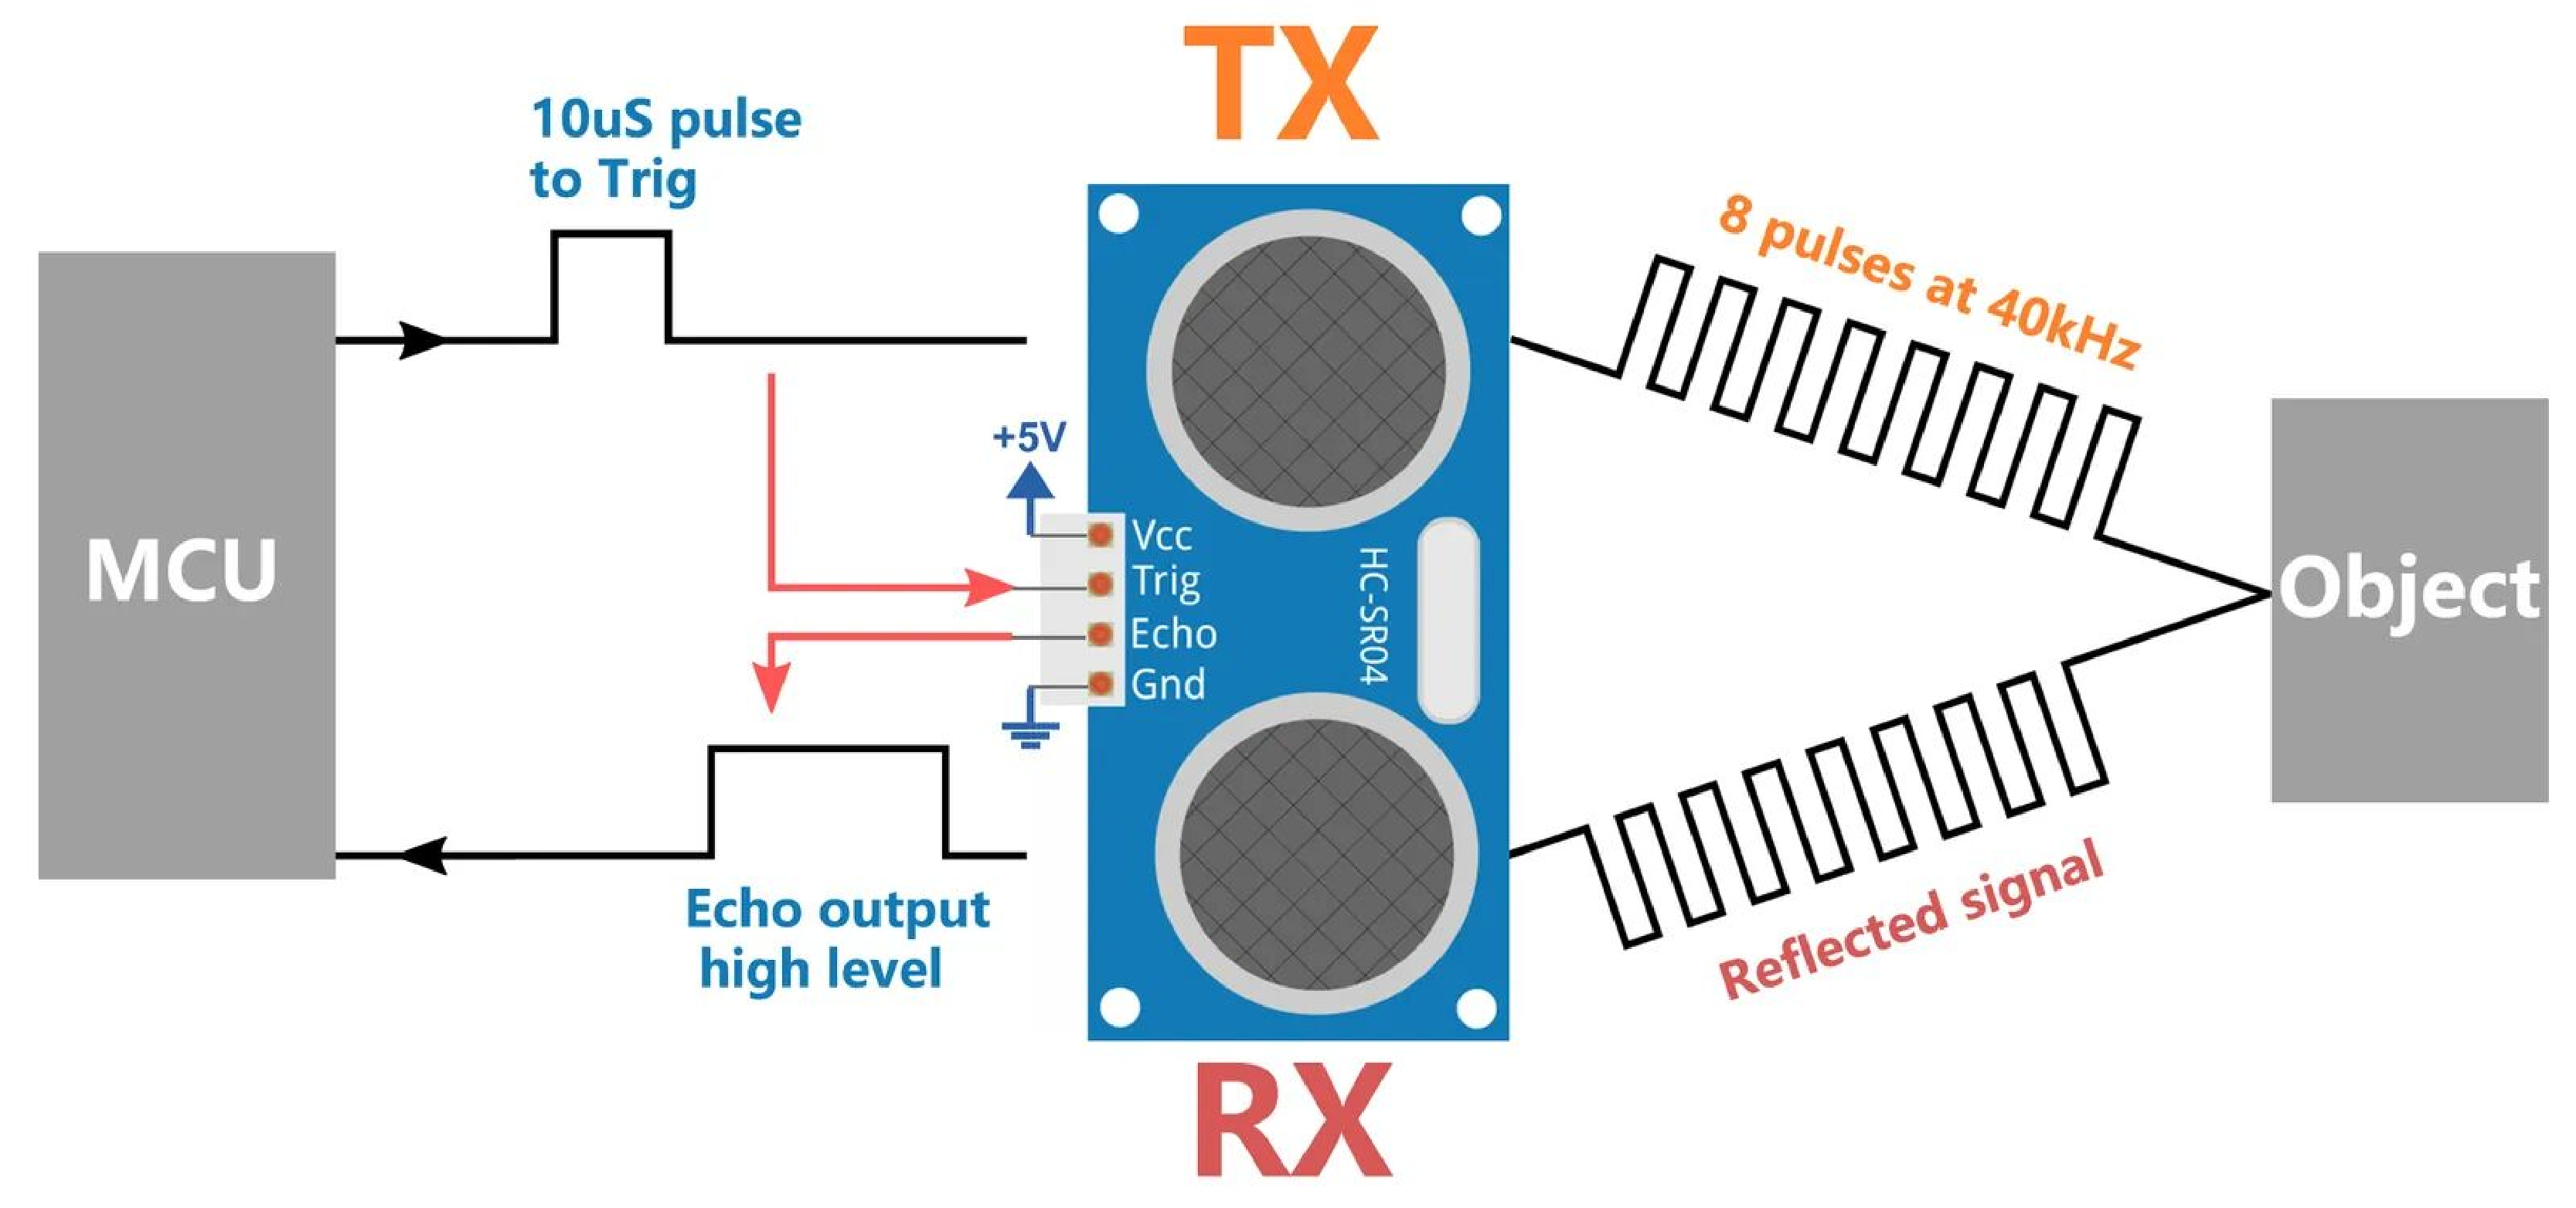
\includegraphics[width=0.8\textwidth]{images/ultrasonic_prin.pdf}
\floatnotes{}
%\label{fig:}
\caption{Ultraschallmodul Prinzip}
\end{figure}

Sensor ist wie ein Fledermaus, die Schallwellen aussendet, um sich zu
orientieren. Wenn du auf einen Knopf drückst (das ist das 10
Mikrosekunden lange Signal), sagst du der >>Fledermaus-Sensor<<, dass
sie ihre >>Ultraschallrufe<< aussenden soll. Diese >>Rufe<< sind sehr,
sehr hoch, viel höher als jedes Geräusch, das wir hören können, und sie
passieren ganz schnell hintereinander, genau 8 Mal in einem winzigen
Moment.

Das ist, als würdest du schnell hintereinander 8 Mal in die Hände
klatschen, nur dass es so schnell und so hoch ist, dass niemand es hören
kann außer der Sensor selbst. Diese speziellen Klatschgeräusche helfen
der >>Fledermaus-Sensor<<, zu erkennen, wie weit Dinge von ihr entfernt
sind, ähnlich wie echte Fledermäuse es tun, wenn sie durch die Nacht
fliegen.

\begin{itemize}
\item
  \textbf{10 Mikrosekunden (10us)}: Der Sensor wird durch ein Signal von
  10 Mikrosekunden (10us) Länge aktiviert, das ist der Startimpuls. Es
  ist wie das Drücken eines Startknopfes, aber es passiert super
  schnell, in nur einem winzigen Bruchteil einer Sekunde.
\item
  \textbf{8-Zyklus-Burst}: sendet einen Ultraschall-Burst, besteht aus 8
  Ultraschallwellen bei einer Frequenz von 40 kHz, um Entfernungen zu
  messen. Stell dir vor, du klatschst 8 Mal ganz schnell hintereinander
  in die Hände -- so ähnlich macht es der Sensor mit Schallwellen, die
  wir aber nicht hören können.
\item
  \textbf{40 kHz (Kilohertz)}: Das ist die Höhe oder Frequenz des
  Ultraschallsignals, das der Sensor aussendet. Kilohertz ist eine
  Einheit, die verwendet wird, um zu beschreiben, wie hoch oder tief ein
  Ton ist. 40 kHz bedeutet, der Ton schwingt 40.000 Mal pro Sekunde. Das
  ist viel höher als das, was das menschliche Ohr hören kann.
\end{itemize}

Das \textbf{menschliche Gehör} kann normalerweise Töne in einem Bereich
von etwa \textbf{20 Hertz (Hz) bis 20.000 Hertz (20 kHz)} wahrnehmen.
Das bedeutet, alles, was unter 20 Hz oder über 20 kHz liegt, können wir
nicht hören. Der Ultraschall, den der Sensor verwendet, liegt also weit
außerhalb des Bereichs, den unsere Ohren erfassen können, weil er bei 40
kHz ist, also doppelt so hoch wie die obere Grenze unseres Hörvermögens.

\hypertarget{berechne-die-entfernung-zu-einem-objekt}{%
\subsubsection{Berechne die Entfernung zu einem
Objekt}\label{berechne-die-entfernung-zu-einem-objekt}}

Angenommen, wir messen die Entfernung zu einem Objekt, das 1 Meter
entfernt ist.

\begin{enumerate}
\def\labelenumi{\arabic{enumi}.}

\item
  \textbf{Trigger-Signal senden}:

  \begin{itemize}
  
  \item
    Der Sensor erhält über den TRIG-Pin ein 10 Mikrosekunden (µs) hohes
    Signal, was ihn veranlasst, einen 8-Zyklus-Burst von
    Ultraschallwellen mit einer Frequenz von 40 kHz zu senden.
  \end{itemize}
\item
  \textbf{Echo-Signal empfangen}:

  \begin{itemize}
  
  \item
    Nach dem Senden des Bursts wartet der Sensor auf das Echo, also das
    Zurückkommen der Ultraschallwellen, nachdem diese vom Objekt
    reflektiert wurden.
  \end{itemize}
\item
  \textbf{Zeitmessung}:

  \begin{itemize}
  
  \item
    Die Zeit vom Senden bis zum Empfangen des Echos wird gemessen.
    Nehmen wir an, die gemessene Zeit (Echo-Zeit) beträgt 5.82
    Millisekunden (ms).
  \end{itemize}
\item
  \textbf{Entfernung berechnen}:

  \begin{itemize}
  
  \item
    Die Entfernung wird mit der Formel berechnet:
  \item
    $\text{Entfernung} = \frac{\text{Zeit des hohen Niveaus} \times \text{Schallgeschwindigkeit}}{2}$
  \item
    Die Schallgeschwindigkeit in Luft beträgt etwa 340 Meter pro Sekunde
    (M/S). Da unsere Zeit in Millisekunden gemessen wurde, müssen wir
    sie in Sekunden umrechnen, um sie in die Formel einzusetzen (1 ms =
    0.001 Sekunden).
  \end{itemize}
\item
  \textbf{Rechnung}:

  \begin{itemize}
  
  \item
    Umrechnung der Echo-Zeit in Sekunden:
    $5.82 \text{ ms} = 0.00582 \text{ s}$.
  \item
    Einsetzen in die Formel:
  \item
    $\text{Entfernung} = \frac{0.00582 \text{ s} \times 340 \text{ m/s}}{2} = \frac{1.9788 \text{ m}}{2} = 0.9894 \text{ m}$
  \end{itemize}
\end{enumerate}

\hypertarget{keywords-ultraschall}{%
\subsubsection{Keywords Ultraschall}\label{keywords-ultraschall}}

\hypertarget{frequenz}{%
\paragraph{Frequenz}\label{frequenz}}

Die Frequenz beschreibt, wie oft eine Schallwelle (oder jede Art von
Welle) in einer Sekunde schwingt. Sie bestimmt die Tonhöhe eines
Geräusches: je höher die Frequenz, desto höher der Ton.

\hypertarget{huxf6rbarkeit}{%
\paragraph{Hörbarkeit}\label{hoerbarkeit}}

Hörbarkeit bezieht sich darauf, ob ein Geräusch in dem Frequenzbereich
liegt, den das menschliche Ohr wahrnehmen kann, typischerweise zwischen
20 Hz und 20.000 Hz (20 kHz).

\hypertarget{schallwellen}{%
\paragraph{Schallwellen}\label{schallwellen}}

Schallwellen sind Schwingungen, die sich durch die Luft oder ein anderes
Medium ausbreiten und von unserem Ohr als Geräusche wahrgenommen werden
können.

\hypertarget{hertz-hz}{%
\paragraph{Hertz (Hz)}\label{hertz-hz}}

Hertz ist die Einheit für Frequenz im Internationalen Einheitensystem
(SI) und beschreibt, wie viele Schwingungen (Zyklen) pro Sekunde
stattfinden.

\hypertarget{huxf6rschwelle}{%
\paragraph{Hörschwelle}\label{hoerschwelle}}

Die Hörschwelle ist die leiseste Lautstärke eines Tons, die gerade noch
gehört werden kann. Sie variiert je nach Frequenz des Tons und von
Person zu Person.

\hypertarget{ultraschall}{%
\paragraph{Ultraschall}\label{ultraschall}}

Ultraschall bezeichnet Schallwellen, die eine höhere Frequenz haben als
der hörbare Bereich für Menschen (über 20 kHz). Sie werden in der
Medizin für bildgebende Verfahren und in anderen Technologien verwendet.

\hypertarget{infraschall}{%
\paragraph{Infraschall}\label{infraschall}}

Infraschall umfasst Frequenzen unterhalb des menschlichen Hörbereichs
(weniger als 20 Hz) und kann von einigen Tieren wahrgenommen werden oder
tritt bei natürlichen Phänomenen wie Erdbeben auf.

\hypertarget{dezibel-db}{%
\paragraph{Dezibel (dB)}\label{dezibel-db}}

Dezibel ist eine Maßeinheit für die Lautstärke (Schalldruckpegel) eines
Geräusches. Sie hilft, die große Spanne an Hörbarkeit menschlichen
Hörens quantitativ zu erfassen.

\hypertarget{schallgeschwindigkeit}{%
\paragraph{Schallgeschwindigkeit}\label{schallgeschwindigkeit}}

Die Schallgeschwindigkeit ist die Geschwindigkeit, mit der sich
Schallwellen durch ein Medium (wie Luft, Wasser oder Stahl) ausbreiten.
In Luft beträgt sie etwa 343 Meter pro Sekunde bei Raumtemperatur.

\hypertarget{echoortung-und-sonar}{%
\paragraph{Echoortung und Sonar}\label{echoortung-und-sonar}}

Echoortung ist die Fähigkeit einiger Tiere (wie Fledermäuse und
Delfine), die Umgebung zu erkunden, indem sie Schall aussenden und das
Echo analysieren. Sonar ist eine technologische Anwendung dieses
Prinzips, das unter Wasser verwendet wird.

\hypertarget{schallisolierung-und-raumakustik}{%
\paragraph{Schallisolierung und
Raumakustik}\label{schallisolierung-und-raumakustik}}

Schallisolierung bezieht sich auf Techniken, um die Übertragung von
Schall von einem Raum zum anderen zu verhindern. Raumakustik beschäftigt
sich mit der Optimierung von Klangqualität und -verteilung in einem
Raum.

\hypertarget{ultraschallbildgebung-sonographie}{%
\paragraph{Ultraschallbildgebung
(Sonographie)}\label{ultraschallbildgebung-sonographie}}

Ultraschallbildgebung ist ein medizinisches Verfahren, das
Ultraschallwellen nutzt, um Bilder vom Inneren des Körpers zu erzeugen,
z.B. um ein ungeborenes Baby im Mutterleib zu sehen.

\hypertarget{schallausbreitung-in-verschiedenen-medien}{%
\paragraph{Schallausbreitung in verschiedenen
Medien}\label{schallausbreitung-in-verschiedenen-medien}}

Schallwellen breiten sich unterschiedlich in verschiedenen Medien (Luft,
Wasser, Festkörper) aus, beeinflusst durch Faktoren wie Dichte und
Elastizität des Mediums.

\hypertarget{frequenzmodulation-und--demodulation}{%
\paragraph{Frequenzmodulation und
-demodulation}\label{frequenzmodulation-und--demodulation}}

Frequenzmodulation (FM) ist eine Technik, bei der die Frequenz einer
Welle geändert wird, um Informationen zu übertragen. Demodulation ist
der umgekehrte Prozess, bei dem die ursprüngliche Information aus der
modulierten Welle zurückgewonnen wird.

\hypertarget{dopplereffekt}{%
\paragraph{Dopplereffekt}\label{dopplereffekt}}

Der Dopplereffekt tritt auf, wenn sich eine Schallquelle relativ zu
einem Beobachter bewegt, was eine wahrgenommene Änderung der Frequenz
des Schalls zur Folge hat (z.B. das An- und Abschwellen des Geräusches
eines vorbeifahrenden Krankenwagens).

\hypertarget{mathematischen-zugang-ultraschall}{%
\subsubsection{Mathematischen Zugang
Ultraschall}\label{mathematischen-zugang-ultraschall}}

\hypertarget{frequenz-f}{%
\paragraph{\texorpdfstring{Frequenz
($f$)}{Frequenz (f)}}\label{frequenz-f}}

\begin{itemize}

\item
  \textbf{Formel}: $f = \frac{1}{T}$, wobei $T$ die Periodendauer
  ist (die Zeit für eine vollständige Schwingung/Zyklus).
\end{itemize}

\hypertarget{huxf6rbarkeit-1}{%
\paragraph{Hörbarkeit}\label{hoerbarkeit-1}}

\begin{itemize}

\item
  Der hörbare Bereich für Menschen liegt zwischen 20 Hz und 20.000 Hz.
  Frequenzen innerhalb dieses Bereichs sind hörbar, Frequenzen außerhalb
  dieses Bereichs sind entweder Ultraschall (\textgreater{} 20 kHz) oder
  Infraschall (\textless{} 20 Hz).
\end{itemize}

\hypertarget{schallwellen-1}{%
\paragraph{Schallwellen}\label{schallwellen-1}}

\begin{itemize}

\item
  \textbf{Geschwindigkeit ($v$) einer Welle}: $v = f \lambda$, wobei
  $\lambda$ die Wellenlänge ist.
\item
  \textbf{Schallgeschwindigkeit in Luft}: etwa 343 m/s bei 20 °C.
\end{itemize}

\hypertarget{hertz-hz-1}{%
\paragraph{Hertz (Hz)}\label{hertz-hz-1}}

\begin{itemize}

\item
  Einheit für Frequenz, 1 Hz = 1 Schwingung pro Sekunde.
\end{itemize}

\hypertarget{huxf6rschwelle-1}{%
\paragraph{Hörschwelle}\label{hoerschwelle-1}}

\begin{itemize}

\item
  Die Hörschwelle variiert je nach Frequenz, wobei etwa 0 dB SPL
  (Schalldruckpegel) für Frequenzen um 1 kHz als leiseste hörbare Töne
  für Menschen gelten.
\end{itemize}

\hypertarget{ultraschall-und-infraschall}{%
\paragraph{Ultraschall und
Infraschall}\label{ultraschall-und-infraschall}}

\begin{itemize}

\item
  \textbf{Ultraschall}: Frequenzen \textgreater{} 20 kHz, nicht hörbar
  für Menschen.
\item
  \textbf{Infraschall}: Frequenzen \textless{} 20 Hz, ebenfalls nicht
  hörbar für Menschen.
\end{itemize}

\hypertarget{dezibel-db-1}{%
\paragraph{Dezibel (dB)}\label{dezibel-db-1}}

\begin{itemize}

\item
  \textbf{Formel zur Berechnung des Schalldruckpegels}:
  $L = 20 \log_{10}(\frac{p}{p_0})$, wobei $p$ der Schalldruck und
  $p_0$ der Referenzschalldruck (üblicherweise 20 µPa in Luft) ist.
\end{itemize}

\hypertarget{schallgeschwindigkeit-1}{%
\paragraph{Schallgeschwindigkeit}\label{schallgeschwindigkeit-1}}

\begin{itemize}

\item
  Abhängig vom Medium. In Luft etwa 343 m/s, in Wasser etwa 1.483 m/s
  und in Stahl etwa 5.960 m/s.
\end{itemize}

\hypertarget{echoortung-und-sonar-1}{%
\paragraph{Echoortung und Sonar}\label{echoortung-und-sonar-1}}

\begin{itemize}

\item
  \textbf{Entfernungsbestimmung}: $D = \frac{1}{2} t v$, wobei $t$
  die Zeit zwischen Aussenden und Empfangen des Echos ist und $v$ die
  Schallgeschwindigkeit im Medium.
\end{itemize}

\hypertarget{frequenzmodulation-und--demodulation-1}{%
\paragraph{Frequenzmodulation und
-demodulation}\label{frequenzmodulation-und--demodulation-1}}

\begin{itemize}

\item
  \textbf{Frequenzmodulation (FM)}:
  $f(t) = f_c + \Delta f \sin(2 \pi f_m t)$, wobei $f_c$ die
  Trägerfrequenz, $\Delta f$ die Frequenzabweichung und $f_m$ die
  Modulationsfrequenz ist.
\end{itemize}

\hypertarget{dopplereffekt-1}{%
\paragraph{Dopplereffekt}\label{dopplereffekt-1}}

\begin{itemize}

\item
  \textbf{Formel für bewegten Beobachter}:
  $f' = f \left(\frac{v \pm v_o}{v \mp v_s}\right)$, wobei $f'$ die
  wahrgenommene Frequenz, $f$ die ursprüngliche Frequenz, $v$ die
  Schallgeschwindigkeit, $v_o$ die Geschwindigkeit des Beobachters und
  $v_s$ die Geschwindigkeit der Quelle ist. Pluszeichen wird
  verwendet, wenn sich Beobachter und Quelle einander nähern,
  Minuszeichen, wenn sie sich voneinander entfernen.
\end{itemize}

\hypertarget{funktionsprinzip-ir-hindernisvermeidungsmodul}{%
\subsection{Funktionsprinzip
IR-Hindernisvermeidungsmodul}\label{funktionsprinzip-ir-hindernisvermeidungsmodul}}

Stell dir vor, das IR-Hindernisvermeidungsmodul ist wie ein Spiel mit
einem Ball, den du wirfst und der zurückkommt, wenn er auf etwas trifft.
Nur dass hier statt einem Ball Infrarotlicht verwendet wird, das wir
nicht sehen können.

\begin{itemize}
\item
  \textbf{IR-Sender-Empfänger-Paar}: Das Modul hat zwei Hauptteile,
  ähnlich wie du zwei Hände hast -- eine zum Werfen des Balls (das ist
  der IR-Sender) und eine zum Fangen (das ist der IR-Empfänger).
\item
  \textbf{Sender emittiert Infrarotlicht}: Der Sender im Modul >>wirft<<
  Infrarotlicht >>Bälle<< aus. Infrarotlicht ist eine Art Licht, das wir
  nicht mit unseren Augen sehen können, aber es ist überall um uns
  herum, zum Beispiel kommt es von der Fernbedienung deines Fernsehers.
\item
  \textbf{Licht trifft auf Hindernisse}: Wenn das Infrarotlicht auf ein
  Hindernis vor dem Modul trifft -- sagen wir, ein Buch auf dem Boden
  oder eine Wand --, wird das Licht von diesem Hindernis
  >>zurückgeworfen<< wie ein Ball, der von einer Wand abprallt.
\item
  \textbf{Empfänger detektiert reflektiertes Licht}: Der IR-Empfänger im
  Modul wartet darauf, das zurückgeworfene Infrarotlicht >>zu fangen<<.
  Wenn er das Licht >>fängt<<, weiß das Modul, dass etwas da ist -- ein
  Hindernis.
\item
  \textbf{Ausgabe eines niedrigen Signals}: Sobald der Empfänger das
  reflektierte Licht erfasst, sagt das Modul: >>Huch, da ist etwas im
  Weg!<< und sendet ein spezielles Signal aus, ein >>niedriges Signal<<,
  um zu zeigen, dass ein Hindernis erkannt wurde. Dieses Signal kann
  dann von einem Computer, einem Roboter oder einem anderen Gerät
  verwendet werden, um zu entscheiden, was als Nächstes zu tun ist, wie
  zum Beispiel anzuhalten oder die Richtung zu ändern.
\end{itemize}

\textbf{Mathematische Annäherung} nutzen, um zu verstehen, wie die
Entfernungsmessung und die Auswirkung der Objektfarbe auf die
Reflexionsniveaus funktionieren. Das Modul verwendet Infrarotlicht, um
Objekte zu erkennen, indem es Licht aussendet und das von Objekten
reflektierte Licht misst. Die Zeit vom Aussenden bis zum Empfang des
reflektierten Lichts gibt Aufschluss über die Entfernung zum Objekt.

\hypertarget{grundlagen-der-entfernungsmessung}{%
\subsubsection{Grundlagen der
Entfernungsmessung}\label{grundlagen-der-entfernungsmessung}}

Die Grundidee hinter der Entfernungsmessung mit einem IR-Sensor basiert
auf der Lichtgeschwindigkeit und der Zeit, die das Licht benötigt, um
zum Sensor zurückzukehren. Für präzise Messungen in kurzen Entfernungen,
wie sie bei IR-Hindernisvermeidungsmodulen üblich sind, berücksichtigt
man die Geschwindigkeit des Lichts und die Verarbeitungszeit des
Sensors.

\hypertarget{einfluss-der-objektfarbe}{%
\paragraph{Einfluss der Objektfarbe}\label{einfluss-der-objektfarbe}}

Die Reflexionseigenschaften von Objekten beeinflussen, wie viel Licht
zum Sensor zurückkehrt. Dunklere Farben absorbieren mehr Licht und
reflektieren weniger, was zu einem schwächeren Signal führt. Helle
Farben reflektieren mehr Licht und führen zu einem stärkeren Signal. Das
Modul misst die Intensität des reflektierten Lichts, um zu bestimmen, ob
ein Objekt innerhalb des Erfassungsbereichs liegt.

\hypertarget{mathematische-betrachtung-der-reflexionsniveaus}{%
\paragraph{Mathematische Betrachtung der
Reflexionsniveaus}\label{mathematische-betrachtung-der-reflexionsniveaus}}

Die Intensität des reflektierten Lichts ($I$) kann durch das
Lambert-Beersche Gesetz angenähert werden, das die Absorption und
Reflexion von Licht durch ein Material beschreibt:

$I = I_0 \, e^{-\alpha d}$

\begin{itemize}

\item
  $I_0$ ist die ursprüngliche Intensität des ausgesendeten Lichts,
\item
  $\alpha$ ist der Absorptionskoeffizient des Materials (höher für
  dunklere Objekte),
\item
  $d$ ist die Dicke des Materials oder die Distanz, die das Licht
  durch das Objekt zurücklegt.
\end{itemize}

Für das IR-Hindernisvermeidungsmodul ist $d$ die Entfernung zum
Objekt, und der Absorptionskoeffizient kann als Maß für die Farbe oder
Reflexionsfähigkeit des Objekts angesehen werden.

\hypertarget{entfernungsberechnung}{%
\paragraph{Entfernungsberechnung}\label{entfernungsberechnung}}

Angenommen, ein IR-Sensor misst die Zeit $t = 1 \times 10^{-4}$
Sekunden für das Licht, um von einem Objekt reflektiert zu werden und
zurückzukehren. Die Entfernung ($d$) zum Objekt kann berechnet werden
als:

$d = \frac{c \cdot t}{2}$

Wobei $c$ die Lichtgeschwindigkeit ist. Für kurze Distanzen und die
schnelle Reflexion von Infrarotlicht ist jedoch die genaue
Geschwindigkeit des Lichts oft weniger relevant als die direkte Messung
der Zeit und die Kalibrierung des Sensors.

Infrarot-Hindernisvermeidungsmodule nutzen die Prinzipien der
Lichtreflexion und -absorption, um Objekte innerhalb eines bestimmten
Bereichs zu erkennen. Die Farbe des Objekts beeinflusst die
Reflexionsniveaus, und die Sensorik ist darauf ausgelegt, diese
Unterschiede zu erfassen und zu interpretieren, um Hindernisse zu
identifizieren. Die mathematische Modellierung dieser Prozesse
ermöglicht ein tieferes Verständnis ihrer Funktionsweise und der
Faktoren, die die Sensorleistung beeinflussen.

\hypertarget{effektive-winkel-von-35}{%
\subsubsection{effektive Winkel von 35°}\label{effektive-winkel-von-35}}

Der \textbf{effektive Winkel von 35°} bei einem
IR-Hindernisvermeidungsmodul bezieht sich auf den Winkelbereich,
innerhalb dessen das Modul effektiv Hindernisse erkennen kann.

\begin{itemize}
\item
  \textbf{Fokussierte Erkennung}: Der Sensor kann Objekte innerhalb
  eines Kegels erkennen, der im Zentrum eine Spitze hat (dort, wo der
  Sensor montiert ist) und sich mit einem Öffnungswinkel von 35° nach
  außen ausweitet. Dies begrenzt die Erkennungszone auf einen
  spezifischen Bereich vor dem Sensor.
\item
  \textbf{Planung der Sensorplatzierung}: Für eine umfassende Abdeckung
  rund um den Roboter könnten mehrere Sensoren benötigt werden, da jeder
  Sensor nur Hindernisse innerhalb seines effektiven Winkels von 35°
  erkennen kann. Durch strategische Platzierung dieser Sensoren kann ein
  Roboter eine 360°-Hinderniserkennung erreichen.
\item
  \textbf{Navigationsgenauigkeit}: Der effektive Winkel beeinflusst, wie
  genau der Roboter seine Umgebung >>sieht<<. Ein schmalerer Winkel
  bietet eine genauere Erkennung in die Tiefe des Feldes, während ein
  breiterer Winkel eine breitere, aber weniger präzise Erkennung
  ermöglicht. Mit 35° bietet der Sensor eine ausgewogene Mischung aus
  Breite und Genauigkeit.
\item
  \textbf{Vermeidungsstrategien}: Der Roboter verwendet die
  Informationen aus dem Sensor, um Kollisionen zu vermeiden. Mit einem
  effektiven Winkel von 35° muss der Roboter möglicherweise seine Route
  anpassen, wenn ein Hindernis innerhalb dieses Bereichs erkannt wird,
  was die Bewegungsplanung und Strategie zur Hindernisvermeidung
  beeinflusst.
\end{itemize}

Die Montage der IR-Hindernisvermeidungsmodul in einem Winkel von 35°
nach vorne außen, zusammen mit einem zentralen Ultraschallsensor, eine
kluge Wahl für die Optimierung der Hinderniserkennung und -vermeidung
bei einem Rover ist. Diese Anordnung erhöht die räumliche Wahrnehmung
und ermöglicht eine effektivere Navigation in komplexen Umgebungen.

\hypertarget{keywords-infrarotlicht-ir}{%
\subsubsection{Keywords Infrarotlicht
(IR)}\label{keywords-infrarotlicht-ir}}

\begin{enumerate}
\def\labelenumi{\arabic{enumi}.}
\item
  \textbf{Wellenlänge}: Der Abstand zwischen zwei aufeinanderfolgenden
  Wellenbergen oder -tälern in einer Welle. Bestimmt Farbe und Energie
  des Lichts.
\item
  \textbf{Sichtbares Licht}: Der Teil des elektromagnetischen Spektrums,
  den das menschliche Auge sehen kann, von Violett bis Rot.
\item
  \textbf{Elektromagnetisches Spektrum}: Die gesamte Bandbreite
  elektromagnetischer Wellen, von sehr kurzen Gammastrahlen bis zu sehr
  langen Radiowellen, einschließlich sichtbarem Licht.
\item
  \textbf{Infrarotlicht (IR)}: Lichtwellen, die länger als rotes Licht
  sind und von uns als Wärme gefühlt, aber nicht gesehen werden können.
\item
  \textbf{Ultraviolettes Licht (UV)}: Lichtwellen, die kürzer als
  violettes Licht sind und Hautbräunung oder -schäden verursachen
  können.
\item
  \textbf{Nanometer (nm)}: Eine Einheit zur Messung der Wellenlänge des
  Lichts, wobei 1 Nanometer einem milliardsten Meter entspricht.
\item
  \textbf{Photonen}: Teilchen, die Lichtwellen tragen. Sie sind die
  kleinsten Energiequanten im Licht.
\item
  \textbf{Farbspektrum}: Die Reihe von Farben, die durch das Aufteilen
  von Licht in seine einzelnen Wellenlängen entsteht, z.B. durch ein
  Prisma.
\item
  \textbf{Transparenz und Opazität}: Eigenschaften von Materialien, die
  bestimmen, ob Licht durch sie hindurchgehen kann (transparent) oder
  nicht (opak).
\item
  \textbf{Reflexion und Brechung}: Reflexion ist das Zurückwerfen von
  Licht von einer Oberfläche. Brechung ist die Änderung der Richtung des
  Lichts, wenn es von einem Medium in ein anderes übergeht.
\item
  \textbf{Lichtabsorption}: Wenn Materialien Licht aufnehmen und in eine
  andere Energieform umwandeln, oft Wärme.
\item
  \textbf{Prisma und Lichtdispersion}: Ein Prisma kann Licht in sein
  Farbspektrum aufteilen, indem es die verschiedenen Wellenlängen
  unterschiedlich bricht.
\item
  \textbf{Nachtsicht und Infrarottechnologien}: Technologien, die
  Infrarotlicht nutzen, um in der Dunkelheit zu sehen oder Bilder zu
  erzeugen.
\item
  \textbf{Wärmebildtechnik}: Eine Technik, die Temperaturunterschiede in
  einer Szene erfasst und sie in ein sichtbares Bild umwandelt,
  basierend auf Infrarotstrahlung.
\item
  \textbf{Lichtquellen}: Objekte oder Geräte, die Licht aussenden, wie
  die Sonne, Glühbirnen oder Laser.
\item
  \textbf{Farbtemperatur}: Ein Maß für die Lichtfarbe, gemessen in
  Kelvin (K), das angibt, ob das Licht eher warm (gelblich) oder kühl
  (bläulich) ist.
\item
  \textbf{Lasertechnologie}: Technologie, die Licht durch einen Prozess
  der optischen Verstärkung erzeugt, was zu einem sehr engen und
  fokussierten Lichtstrahl führt.
\item
  \textbf{Holographie}: Eine Technik zur Erzeugung dreidimensionaler
  Bilder mit Laserlicht.
\item
  \textbf{Elektromagnetische Wellentheorie}: Die Theorie, die die
  Ausbreitung elektromagnetischer Wellen, einschließlich Licht, durch
  Raum oder Materie beschreibt.
\end{enumerate}

\hypertarget{mathematischen-zugang-infrarotlicht-ir}{%
\subsubsection{Mathematischen Zugang Infrarotlicht
(IR)}\label{mathematischen-zugang-infrarotlicht-ir}}

\hypertarget{wellenluxe4nge-lambda}{%
\paragraph{\texorpdfstring{1. Wellenlänge
($\lambda$)}{1. Wellenlänge (\textbackslash lambda)}}\label{wellenlaenge-lambda}}

\begin{itemize}

\item
  \textbf{Mathematische Darstellung}: $\lambda = \frac{v}{f}$

  \begin{itemize}
  
  \item
    $v$ ist die Geschwindigkeit der Welle (z.B. Lichtgeschwindigkeit
    im Vakuum, etwa $3 \times 10^8$ m/s).
  \item
    $f$ ist die Frequenz der Welle in Hertz (Hz).
  \end{itemize}
\end{itemize}

\hypertarget{sichtbares-licht-und-elektromagnetisches-spektrum}{%
\paragraph{2. Sichtbares Licht und Elektromagnetisches
Spektrum}\label{sichtbares-licht-und-elektromagnetisches-spektrum}}

\begin{itemize}

\item
  \textbf{Bereich des sichtbaren Lichts}: Etwa 380 nm bis 740 nm.
\item
  \textbf{Umrechnung in Frequenz}: $f = \frac{c}{\lambda}$, wobei
  $c$ die Lichtgeschwindigkeit ist.
\end{itemize}

\hypertarget{infrarotlicht-ir-und-ultraviolettes-licht-uv}{%
\paragraph{3. Infrarotlicht (IR) und Ultraviolettes Licht
(UV)}\label{infrarotlicht-ir-und-ultraviolettes-licht-uv}}

\begin{itemize}

\item
  \textbf{IR-Bereich}: Wellenlängen größer als 740 nm.
\item
  \textbf{UV-Bereich}: Wellenlängen kleiner als 380 nm.
\item
  \textbf{Berechnung der Energie eines Photons}:
  $E = hf = \frac{hc}{\lambda}$, wobei $h$ das Plancksche
  Wirkungsquantum ist.
\end{itemize}

\hypertarget{nanometer-nm}{%
\paragraph{4. Nanometer (nm)}\label{nanometer-nm}}

\begin{itemize}

\item
  \textbf{Umrechnung}: 1 nm = $10^{-9}$ Meter.
\item
  \textbf{Anwendung in Formeln}: Direkte Einsetzung der Wellenlänge in
  nm nach Umrechnung in Meter für physikalische Berechnungen.
\end{itemize}

\hypertarget{transparenz-reflexion-brechung-und-lichtabsorption}{%
\paragraph{5. Transparenz, Reflexion, Brechung, und
Lichtabsorption}\label{transparenz-reflexion-brechung-und-lichtabsorption}}

\begin{itemize}

\item
  \textbf{Brechungsindex}: $n = \frac{c}{v_{medium}}$, wobei
  $v_{medium}$ die Geschwindigkeit des Lichts im Medium ist.
\item
  \textbf{Snelliussches Brechungsgesetz}:
  $n_1 \sin(\theta_1) = n_2 \sin(\theta_2)$, wobei $\theta$ der
  Winkel zur Normalen ist.
\end{itemize}

\hypertarget{prisma-und-lichtdispersion}{%
\paragraph{6. Prisma und
Lichtdispersion}\label{prisma-und-lichtdispersion}}

\begin{itemize}

\item
  \textbf{Dispersion}: Abhängigkeit des Brechungsindex von der
  Wellenlänge, was zu Farbaufspaltung führt.
\end{itemize}

\hypertarget{farbtemperatur}{%
\paragraph{7. Farbtemperatur}\label{farbtemperatur}}

\begin{itemize}

\item
  \textbf{Einheit}: Kelvin (K).
\item
  \textbf{Zusammenhang mit Spektrum}: Höhere Farbtemperaturen
  entsprechen bläulicherem Licht, niedrigere wärmerem Licht.
\end{itemize}

\hypertarget{lasertechnologie-und-holographie}{%
\paragraph{8. Lasertechnologie und
Holographie}\label{lasertechnologie-und-holographie}}

\begin{itemize}

\item
  \textbf{Kohärenz und Monochromasie}: Laserlicht hat sehr enge
  Wellenlängenbereiche, ideal für Interferenz und Holographie.
\end{itemize}

\hypertarget{photonik-und-elektromagnetische-wellentheorie}{%
\paragraph{9. Photonik und Elektromagnetische
Wellentheorie}\label{photonik-und-elektromagnetische-wellentheorie}}

\begin{itemize}

\item
  \textbf{Photonenenergie}: Siehe Formel oben.
\item
  \textbf{Maxwellsche Gleichungen}: Grundlage der elektromagnetischen
  Wellentheorie, beschreiben die Ausbreitung elektromagnetischer Felder.
\end{itemize}

\hypertarget{funktionsprinzip-servo}{%
\subsection{Funktionsprinzip Servo}\label{funktionsprinzip-servo}}

\hypertarget{motor}{%
\paragraph{Motor}\label{motor}}

\begin{itemize}

\item
  Im Servo befindet sich ein Motor, ähnlich denen, die die Räder eines
  Marsrovers antreiben könnten. Dieser Motor ist für die Bewegung
  zuständig.
\end{itemize}

\hypertarget{die-kraft-der-uxfcbersetzung-zahnruxe4der}{%
\paragraph{Die Kraft der Übersetzung:
Zahnräder}\label{die-kraft-der-uebersetzung-zahnraeder}}

\begin{itemize}

\item
  Um die Motorbewegung zu kontrollieren und kraftvoller zu machen, sind
  um den Motor herum Zahnräder angeordnet. Ein großes Zahnrad greift in
  ein kleineres ein, das direkt auf der Motorwelle sitzt. Diese
  Anordnung wandelt die schnelle Drehung des Motors in eine langsamere,
  aber stärkere Bewegung um. Das ist wichtig, weil wir oft wollen, dass
  der Rover präzise und kraftvoll agiert, zum Beispiel beim Bewegen
  seiner Arme oder beim Drehen seines Körpers.
\end{itemize}

\hypertarget{potentiometer-und-steuerungsschaltung}{%
\paragraph{Potentiometer und
Steuerungsschaltung}\label{potentiometer-und-steuerungsschaltung}}

\begin{itemize}

\item
  Ein wichtiger Teil des Servos ist das Potentiometer. Stell dir das
  Potentiometer wie einen kleinen Detektiv vor, der immer genau weiß, in
  welcher Position sich der Servo befindet. Wenn sich der Servo dreht,
  dreht sich auch das Potentiometer und verändert seinen Widerstand.
\item
  Die Steuerungsschaltung im Servo ist wie das Gehirn, das die
  Informationen des Potentiometers liest. Sie versteht die Veränderung
  des Widerstands und weiß dadurch, in welcher Position sich der Servo
  befindet. So kann sie den Servo genau dort anhalten, wo er sein soll.
\end{itemize}

\hypertarget{pulsweitenmodulation-pwm}{%
\paragraph{Pulsweitenmodulation (PWM)}\label{pulsweitenmodulation-pwm}}

\begin{itemize}

\item
  Durch die Anpassung der >>Länge<< (also der Impulse) können wir den
  Servo sehr genau steuern. So können wir dem Rover befehlen, seinen Arm
  genau so zu bewegen, wie wir es möchten, oder sich in eine bestimmte
  Richtung zu drehen.
\end{itemize}

\hypertarget{newton}{%
\subsection{Newton}\label{newton}}

Ein \textbf{Newton} (Symbol: \textbf{N}) ist die SI-Einheit der Kraft.
Sie ist definiert als die Kraft, die erforderlich ist, um einem
Kilogramm Masse eine Beschleunigung von einem Meter pro Sekunde im
Quadrat zu erteilen. Mathematisch ausgedrückt:

$1 \, \text{N} = 1 \, \text{kg} \cdot \text{m} / \text{s}^2$

Das bedeutet, dass ein Newton die Menge an Kraft ist, die benötigt wird,
um ein Objekt mit einer Masse von einem Kilogramm mit einer Rate von
einem Meter pro Sekunde pro Sekunde zu beschleunigen.

\hypertarget{mathematischer-zugang-zu-newton}{%
\subsubsection{Mathematischer Zugang zu
Newton}\label{mathematischer-zugang-zu-newton}}

Die Beziehung zwischen den Grundgrößen in der Physik, wie Masse,
Beschleunigung und Kraft, kann durch das zweite Newtonsche Gesetz
ausgedrückt werden:

$F = m \cdot a$

\begin{itemize}

\item
  $F$ ist die Kraft in Newton,
\item
  $m$ ist die Masse in Kilogramm,
\item
  $a$ ist die Beschleunigung in Metern pro Sekunde im Quadrat
  ($m/s^2$).
\end{itemize}

\hypertarget{rechenbeispiel-kraftberechnung}{%
\paragraph{Rechenbeispiel:
Kraftberechnung}\label{rechenbeispiel-kraftberechnung}}

Angenommen, ein Auto mit einer Masse von 1000 kg soll aus dem Stand
innerhalb von 5 Sekunden auf eine Geschwindigkeit von 10 m/s
beschleunigt werden. Die Beschleunigung ($a$) kann zuerst berechnet
werden als:

$a = \frac{\Delta v}{\Delta t} = \frac{10 \, \text{m/s}}{5 \, \text{s}} = 2 \, \text{m/s}^2$

Dann kann die Kraft ($F$) berechnet werden, die benötigt wird, um
diese Beschleunigung zu erreichen:

$F = m \cdot a = 1000 \, \text{kg} \cdot 2 \, \text{m/s}^2 = 2000 \, \text{N}$

Das bedeutet, dass eine Kraft von 2000 Newton erforderlich ist, um das
Auto unter den gegebenen Bedingungen zu beschleunigen.

\hypertarget{unterschied-zwischen-gewicht-und-masse}{%
\subsubsection{Unterschied zwischen Gewicht und
Masse}\label{unterschied-zwischen-gewicht-und-masse}}

\begin{itemize}

\item
  \textbf{Masse}: Ein Maß für die Menge an Materie in einem Objekt. Die
  Masse ist eine inhärente Eigenschaft eines Objekts und ändert sich
  nicht, unabhängig von der Position im Universum.
\item
  \textbf{Gewicht}: Eine Kraft, die aufgrund der Gravitationsanziehung
  auf eine Masse wirkt. Das Gewicht kann variieren, abhängig von der
  Gravitationsbeschleunigung des Ortes, an dem sich das Objekt befindet.
\end{itemize}

\hypertarget{umrechnung-zwischen-kilogramm-und-newton}{%
\paragraph{Umrechnung zwischen Kilogramm und
Newton}\label{umrechnung-zwischen-kilogramm-und-newton}}

Die Umrechnung zwischen Kilogramm (kg) und Newton (N) hängt von der
Gravitationsbeschleunigung ab. Auf der Erdoberfläche beträgt die
durchschnittliche Gravitationsbeschleunigung etwa
$9,81 \, \text{m/s}^2$.

$1 \, \text{kg} \approx 9,81 \, \text{N}$

Das bedeutet, dass die Gewichtskraft eines Körpers mit der Masse 1 kg
auf der Erdoberfläche etwa 9,81 N beträgt.

\hypertarget{was-ist-gravitationsbeschleunigung}{%
\subsubsection{Was ist
Gravitationsbeschleunigung?}\label{was-ist-gravitationsbeschleunigung}}

Stell dir vor, du lässt einen Ball fallen. Während der Ball fällt, wird
er schneller und schneller. Das liegt daran, dass die Erde eine Art
unsichtbare Kraft hat, die alles zu sich zieht -- wir nennen das
Gravitation. Die Gravitationsbeschleunigung ist ein Maß dafür, wie
schnell etwas durch diese Kraft beschleunigt wird, wenn es fällt.

Die Zahl $9,81 \, \text{m/s}^2$ sagt uns, wie schnell der Ball jedes
Sekunde schneller wird, wenn er fällt. Das bedeutet, am Ende der ersten
Sekunde fällt der Ball mit einer Geschwindigkeit von
$9,81 \, \text{Meter pro Sekunde}$. Nach zwei Sekunden ist er schon
doppelt so schnell, also etwa $19,62 \, \text{Meter pro Sekunde}$, und
so wird er immer schneller, je länger er fällt.

\hypertarget{experiment-freier-fall---volle-und-eine-leere-flasche-gleichzeitig-fallen}{%
\paragraph{Experiment freier Fall - volle und eine leere Flasche
gleichzeitig
fallen}\label{experiment-freier-fall---volle-und-eine-leere-flasche-gleichzeitig-fallen}}

Wenn du eine volle und eine leere Flasche gleichzeitig fallen lässt,
fallen sie tatsächlich mit der gleichen Geschwindigkeit, vorausgesetzt,
dass sie im Vakuum fallen, wo kein Luftwiderstand vorhanden ist. Das
liegt daran, dass die Gravitationsbeschleunigung für alle Objekte an
einem bestimmten Ort gleich ist, unabhängig von ihrer Masse. Dieses
Prinzip wurde von Galileo Galilei durch seine Experimente im 16.
Jahrhundert entdeckt und später von Isaac Newton in seinen
Bewegungsgesetzen formuliert.

In der realen Welt, außerhalb eines Vakuums, spielt jedoch der
Luftwiderstand eine Rolle. Der Luftwiderstand hängt von verschiedenen
Faktoren ab, einschließlich der Form des Objekts und seiner Oberfläche.
Wenn die volle und die leere Flasche genau dieselbe Form und Größe
haben, könnte die volle Flasche schneller fallen als die leere, weil sie
eine größere Masse hat und der Unterschied im Luftwiderstand zwischen
beiden Flaschen nicht ausreicht, um den Fall der schwereren Flasche
signifikant zu verlangsamen. Aber der Unterschied wäre unter normalen
Bedingungen minimal.

In der Praxis bedeutet das, dass, obwohl theoretisch beide Flaschen mit
der gleichen Rate fallen sollten, die volle Flasche aufgrund ihres
größeren Gewichts leicht schneller fallen könnte als die leere Flasche,
besonders wenn die Flaschen nicht perfekt aerodynamisch sind und der
Luftwiderstand eine Rolle spielt.

\hypertarget{keywords-gravitation-newtonsche-gesetze-und-die-grundlegenden-physikalischen-einheiten}{%
\subsubsection{Keywords Gravitation, Newtonsche Gesetze und die
grundlegenden physikalischen
Einheiten}\label{keywords-gravitation-newtonsche-gesetze-und-die-grundlegenden-physikalischen-einheiten}}

\begin{enumerate}
\def\labelenumi{\arabic{enumi}.}

\item
  \textbf{Gravitation}: Anziehungskraft zwischen Massen,
  Gravitationsfeld, Gravitationsgesetz, universelle
  Gravitationskonstante.
\item
  \textbf{Newton}: Isaac Newton, Newtonsche Gesetze der Bewegung,
  Newtonsches Gravitationsgesetz, Einheit der Kraft.
\item
  \textbf{Kraft}: Grundlegende Wechselwirkung, Newton (N), Kraftvektor,
  resultierende Kraft, Zentripetalkraft.
\item
  \textbf{Beschleunigung}: Änderungsrate der Geschwindigkeit, $m/s^2$,
  gleichmäßige Beschleunigung, Gravitationsbeschleunigung.
\item
  \textbf{Masse}: Menge der Materie, Kilogramm (kg), Trägheit,
  Massenerhaltung.
\item
  \textbf{Gewicht}: Kraft aufgrund der Gravitation, Gewichtskraft,
  Unterschied zwischen Masse und Gewicht, $N$ (Newton).
\item
  \textbf{Meter (m)}: Basiseinheit der Länge, Distanzmessung,
  Lichtgeschwindigkeit in Metern pro Sekunde.
\item
  \textbf{Kilogramm (kg)}: Basiseinheit der Masse, internationaler
  Kilogrammprototyp, Masse-Wasser-Äquivalent.
\item
  \textbf{Sekunde (s)}: Basiseinheit der Zeit, Zeitmessung, Frequenz des
  Cäsium-133-Atoms.
\item
  \textbf{Ampere (A)}: Basiseinheit der elektrischen Stromstärke,
  elektrischer Strom, Coulombs pro Sekunde.
\item
  \textbf{Kelvin (K)}: Basiseinheit der Temperatur, absolute
  Temperaturskala, thermodynamische Temperatur.
\item
  \textbf{Mol (mol)}: Basiseinheit der Stoffmenge, Avogadros Zahl,
  Moleküle und Atome.
\item
  \textbf{Candela (cd)}: Basiseinheit der Lichtstärke, Lichtquellen,
  Luminanz.
\item
  \textbf{Fallgesetze}: Freier Fall, Luftwiderstand,
  Terminalgeschwindigkeit.
\item
  \textbf{Impuls und Impulserhaltung}: Impuls als Produkt aus Masse und
  Geschwindigkeit, Erhaltungsgesetz.
\item
  \textbf{Arbeit und Energie}: Arbeitseinheit Joule, kinetische Energie,
  potenzielle Energie, Energieerhaltung.
\item
  \textbf{Drehmoment}: Rotationskraft, Drehmoment und Hebelgesetz,
  $N\cdot m$ (Newtonmeter).
\item
  \textbf{Schwingungen und Wellen}: Periodische Bewegung, Frequenz,
  Wellenlänge, Schallwellen, elektromagnetische Wellen.
\end{enumerate}

\hypertarget{mathematischen-zugang-gravitation-newtonsche-gesetze-und-die-grundlegenden-physikalischen-einheiten}{%
\subsubsection{Mathematischen Zugang Gravitation, Newtonsche Gesetze und
die grundlegenden physikalischen
Einheiten}\label{mathematischen-zugang-gravitation-newtonsche-gesetze-und-die-grundlegenden-physikalischen-einheiten}}

\hypertarget{gravitation}{%
\paragraph{Gravitation}\label{gravitation}}

\begin{itemize}

\item
  \textbf{Newtonsches Gravitationsgesetz}: $F = G \frac{m_1 m_2}{r^2}$

  \begin{itemize}
  
  \item
    \textbf{Beispiel}: Zwei Massen von je 1 kg im Abstand von 1 m
    zueinander üben eine Anziehungskraft von etwa
    $6,674 \times 10^{-11} \, \text{N}$ aus.
  \end{itemize}
\end{itemize}

\hypertarget{newton-1}{%
\paragraph{Newton}\label{newton-1}}

\begin{itemize}

\item
  \textbf{Zweites Newtonsches Gesetz}: $F = m \cdot a$

  \begin{itemize}
  
  \item
    \textbf{Beispiel}: Ein Objekt mit einer Masse von 10 kg, das mit
    $2 \, \text{m/s}^2$ beschleunigt wird, erfährt eine Kraft von
    $20 \, \text{N}$.
  \end{itemize}
\end{itemize}

\hypertarget{kraft}{%
\paragraph{Kraft}\label{kraft}}

\begin{itemize}

\item
  \textbf{Kraftvektor}: $F = m \cdot a$

  \begin{itemize}
  
  \item
    \textbf{Beispiel}: Ein Auto (Masse = 1000 kg) beschleunigt mit
    $1 \, \text{m/s}^2$, die wirkende Kraft ist $1000 \, \text{N}$.
  \end{itemize}
\end{itemize}

\hypertarget{beschleunigung}{%
\paragraph{Beschleunigung}\label{beschleunigung}}

\begin{itemize}

\item
  \textbf{Gleichmäßige Beschleunigung}:
  $a = \frac{\Delta v}{\Delta t}$

  \begin{itemize}
  
  \item
    \textbf{Beispiel}: Ein Auto erhöht seine Geschwindigkeit von 0 auf
    $60 \, \text{km/h}$ (etwa $16,67 \, \text{m/s}$) in 5 Sekunden,
    $a = 3,33 \, \text{m/s}^2$.
  \end{itemize}
\end{itemize}

\hypertarget{masse-und-gewicht}{%
\paragraph{Masse und Gewicht}\label{masse-und-gewicht}}

\begin{itemize}

\item
  \textbf{Gewicht}: $W = m \cdot g$

  \begin{itemize}
  
  \item
    \textbf{Beispiel}: Eine Masse von 50 kg auf der Erde (mit
    $g = 9,81 \, \text{m/s}^2$) hat ein Gewicht von
    $490,5 \, \text{N}$.
  \end{itemize}
\end{itemize}

\hypertarget{meter-und-kilogramm}{%
\paragraph{Meter und Kilogramm}\label{meter-und-kilogramm}}

\begin{itemize}

\item
  \textbf{Längenmessung}: 1 Meter ist die Basislänge.
\item
  \textbf{Masse}: 1 Kilogramm ist die Basismasse.
\end{itemize}

\hypertarget{sekunde-ampere-kelvin-mol-candela}{%
\paragraph{Sekunde, Ampere, Kelvin, Mol,
Candela}\label{sekunde-ampere-kelvin-mol-candela}}

\begin{itemize}

\item
  \textbf{Zeit}: 1 Sekunde ist die Basiseinheit der Zeit.
\item
  \textbf{Stromstärke}: 1 Ampere ist die Basiseinheit der elektrischen
  Stromstärke.
\item
  \textbf{Temperatur}: 1 Kelvin ist die Basiseinheit der Temperatur.
\item
  \textbf{Stoffmenge}: 1 Mol ist die Basiseinheit der Stoffmenge.
\item
  \textbf{Lichtstärke}: 1 Candela ist die Basiseinheit der Lichtstärke.
\end{itemize}

\hypertarget{fallgesetze-und-impulserhaltung}{%
\paragraph{Fallgesetze und
Impulserhaltung}\label{fallgesetze-und-impulserhaltung}}

\begin{itemize}

\item
  \textbf{Freier Fall}: $s = \frac{1}{2} g t^2$

  \begin{itemize}
  
  \item
    \textbf{Beispiel}: Ein Objekt fällt für 2 Sekunden, zurückgelegte
    Strecke ist $19,62 \, \text{m}$.
  \end{itemize}
\end{itemize}

\hypertarget{arbeit-und-energie}{%
\paragraph{Arbeit und Energie}\label{arbeit-und-energie}}

\begin{itemize}

\item
  \textbf{Arbeit}: $W = F \cdot d$

  \begin{itemize}
  
  \item
    \textbf{Beispiel}: Heben eines Objekts (Kraft = 100 N) um 2 Meter
    verrichtet eine Arbeit von $200 \, \text{J}$.
  \end{itemize}
\end{itemize}

\hypertarget{drehmoment}{%
\paragraph{Drehmoment}\label{drehmoment}}

\begin{itemize}

\item
  \textbf{Drehmoment}: $\tau = F \cdot r$

  \begin{itemize}
  
  \item
    \textbf{Beispiel}: Eine Kraft von $10 \, \text{N}$, die im Abstand
    von 0,5 m vom Drehpunkt wirkt, erzeugt ein Drehmoment von
    $5 \, \text{N}\cdot\text{m}$.
  \end{itemize}
\end{itemize}

\hypertarget{schwingungen-und-wellen}{%
\paragraph{Schwingungen und Wellen}\label{schwingungen-und-wellen}}

\begin{itemize}

\item
  \textbf{Frequenz einer Welle}: $f = \frac{1}{T}$

  \begin{itemize}
  
  \item
    \textbf{Beispiel}: Eine Schwingung, die sich alle 0,5 Sekunden
    wiederholt, hat eine Frequenz von $2 \, \text{Hz}$.
  \end{itemize}
\end{itemize}

\hypertarget{gravitationsbeschleunigungen-fuxfcr-erde-mond-und-mars}{%
\subsubsection{Gravitationsbeschleunigungen für Erde, Mond und
Mars}\label{gravitationsbeschleunigungen-fuer-erde-mond-und-mars}}

Die Gravitationsbeschleunigung eines Himmelskörpers hängt hauptsächlich
von zwei Faktoren ab:

\begin{enumerate}
\def\labelenumi{\arabic{enumi}.}
\item
  \textbf{Masse des Himmelskörpers}: Je größer die Masse eines
  Himmelskörpers ist, desto stärker ist seine Gravitationskraft. Nach
  dem Gravitationsgesetz von Newton ist die Gravitationskraft direkt
  proportional zur Masse des Himmelskörpers. Das bedeutet, dass ein
  Planet mit einer höheren Masse eine stärkere Gravitationsanziehung
  hat, was zu einer höheren Gravitationsbeschleunigung führt.
\item
  \textbf{Radius des Himmelskörpers}: Die Gravitationsbeschleunigung
  hängt auch invers quadratisch vom Radius des Himmelskörpers ab. Wenn
  man sich weiter vom Zentrum eines Himmelskörpers entfernt, nimmt die
  Gravitationsbeschleunigung ab. Dies bedeutet, dass bei zwei
  Himmelskörpern mit gleicher Masse der Körper mit dem kleineren Radius
  eine höhere Gravitationsbeschleunigung an seiner Oberfläche haben
  wird, da man näher am Massenzentrum ist.
\end{enumerate}

Mathematisch wird die Gravitationsbeschleunigung ($g$) an der
Oberfläche eines Himmelskörpers durch die Formel

$g = \frac{G \cdot M}{R^2}$

ausgedrückt, wobei:

\begin{itemize}

\item
  $G$ die universelle Gravitationskonstante ist
  ($6,674 \times 10^{-11} \, \text{m}^3 \text{kg}^{-1} \text{s}^{-2}$),
\item
  $M$ die Masse des Himmelskörpers ist,
\item
  $R$ der Radius des Himmelskörpers ist.
\end{itemize}

\begin{lstlisting}[language=Python]
# Gegebene Werte für Erde, Mond und Mars
# Universelle Gravitationskonstante
G = 6.674 * 10**-11  # m^3 kg^-1 s^-2

# Erde
M_Erde = 5.972 * 10**24  # kg
R_Erde = 6.371 * 10**6  # m

# Mond
M_Mond = 7.347 * 10**22  # kg
R_Mond = 1.737 * 10**6  # m

# Mars
M_Mars = 6.417 * 10**23  # kg
R_Mars = 3.3895 * 10**6  # m

# Berechnung der Gravitationsbeschleunigung für Erde, Mond und Mars
g_Erde = (G * M_Erde) / (R_Erde**2)
g_Mond = (G * M_Mond) / (R_Mond**2)
g_Mars = (G * M_Mars) / (R_Mars**2)

# Ausgabe der Gravitationsbeschleunigungen für Erde, Mond und Mars
print("Gravitationsbeschleunigung auf der Erde:", g_Erde, "m/s^2")
print("Gravitationsbeschleunigung auf dem Mond:", g_Mond, "m/s^2")
print("Gravitationsbeschleunigung auf dem Mars:", g_Mars, "m/s^2")
\end{lstlisting}

Die Gravitationsbeschleunigung eines Himmelskörpers hat signifikante
Auswirkungen auf unseren Körper, vor allem in Bezug auf unser Gewicht,
unsere Muskulatur und das Skelettsystem.

\hypertarget{gewichtsunterschiede}{%
\subsubsection{Gewichtsunterschiede}\label{gewichtsunterschiede}}

\begin{itemize}

\item
  \textbf{Erde}: Auf der Erde erfahren wir die
  Gravitationsbeschleunigung, die unser Körper gewohnt ist. Unser
  Gewicht auf der Erde dient als Referenzwert für Vergleiche mit anderen
  Himmelskörpern.
\item
  \textbf{Mond}: Auf dem Mond beträgt die Gravitationsbeschleunigung nur
  etwa 1/6 der Erdbeschleunigung. Das bedeutet, dass eine Person, die
  auf der Erde 60 kg wiegt, auf dem Mond nur etwa 10 kg wiegen würde.
  Die reduzierte Schwerkraft ermöglicht höhere Sprünge und das Tragen
  schwerer Lasten mit weniger Anstrengung.
\item
  \textbf{Mars}: Mit etwa 1/3 der Erdbeschleunigung würde dasselbe
  Individuum auf dem Mars etwa 20 kg wiegen. Obwohl höher als auf dem
  Mond, bietet auch diese Gravitation eine Erleichterung gegenüber der
  Erdschwerkraft.
\end{itemize}

\hypertarget{muskulatur-und-skelettsystem}{%
\paragraph{Muskulatur und
Skelettsystem}\label{muskulatur-und-skelettsystem}}

\begin{itemize}

\item
  \textbf{Langfristige Auswirkungen in niedriger Schwerkraft}: Ein
  längerer Aufenthalt in Umgebungen mit geringerer Gravitation (wie auf
  dem Mond oder Mars) kann zu Muskelatrophie und Knochenschwund führen,
  da die konstante Notwendigkeit, gegen die Schwerkraft zu arbeiten, als
  natürlicher Widerstand für den Erhalt von Muskel- und Knochenstärke
  entfällt.
\item
  \textbf{Anpassung}: Astronauten, die längere Zeit im Weltraum
  verbringen, wo die Schwerkraft nahezu null ist, zeigen signifikanten
  Verlust an Muskelmasse und Knochendichte. Um dem entgegenzuwirken,
  sind regelmäßige Übungen mit Widerstandsgeräten notwendig, um die
  Auswirkungen der Schwerelosigkeit zu minimieren.
\end{itemize}

\hypertarget{physiologische-anpassungen}{%
\paragraph{Physiologische
Anpassungen}\label{physiologische-anpassungen}}

\begin{itemize}

\item
  \textbf{Herz-Kreislauf-System}: Die geringere Schwerkraft auf dem Mond
  oder Mars würde auch das Herz-Kreislauf-System beeinflussen, da das
  Herz nicht so stark pumpen muss, um Blut durch den Körper zu
  zirkulieren. Langfristig könnte dies zu Veränderungen in der Herzgröße
  und -funktion führen.
\item
  \textbf{Gleichgewichtssinn und Orientierung}: Die Veränderung der
  Gravitationsbeschleunigung kann auch den Gleichgewichtssinn
  beeinträchtigen. Das vestibuläre System im Ohr, das für die
  Orientierung und das Gleichgewicht verantwortlich ist, muss sich an
  die neue Umgebung anpassen, was anfangs zu Desorientierung führen
  kann.
\end{itemize}

\hypertarget{si-einheiten}{%
\subsection{SI-Einheiten}\label{si-einheiten}}

Das Internationale Einheitensystem (SI) definiert sieben
Basis-Einheiten, von denen alle anderen Einheiten abgeleitet werden:

\begin{enumerate}
\def\labelenumi{\arabic{enumi}.}

\item
  \textbf{Meter (m)} - Einheit der Länge
\item
  \textbf{Kilogramm (kg)} - Einheit der Masse
\item
  \textbf{Sekunde (s)} - Einheit der Zeit
\item
  \textbf{Ampere (A)} - Einheit der elektrischen Stromstärke
\item
  \textbf{Kelvin (K)} - Einheit der thermodynamischen Temperatur
\item
  \textbf{Mol (mol)} - Einheit der Stoffmenge
\item
  \textbf{Candela (cd)} - Einheit der Lichtstärke
\end{enumerate}

\hypertarget{mathematischer-zugang-zu-si-einheiten}{%
\subsubsection{Mathematischer Zugang zu
SI-Einheiten}\label{mathematischer-zugang-zu-si-einheiten}}

\hypertarget{meter-m---einheit-der-luxe4nge}{%
\paragraph{Meter (m) - Einheit der
Länge}\label{meter-m---einheit-der-laenge}}

\begin{itemize}

\item
  \textbf{Beispiel}: Ein Raum ist 5 m lang. Wenn man den Boden mit
  Fliesen auslegt, die 0,25 m breit sind, benötigt man
  $5 \, \text{m} / 0,25 \, \text{m} = 20$ Fliesen für eine Reihe.
\end{itemize}

\hypertarget{kilogramm-kg---einheit-der-masse}{%
\paragraph{Kilogramm (kg) - Einheit der
Masse}\label{kilogramm-kg---einheit-der-masse}}

\begin{itemize}

\item
  \textbf{Beispiel}: Ein Sack Reis wiegt 25 kg. Wenn eine Person täglich
  0,5 kg Reis verbraucht, reicht der Sack für
  $25 \, \text{kg} / 0,5 \, \text{kg/Tag} = 50$ Tage.
\end{itemize}

\hypertarget{sekunde-s---einheit-der-zeit}{%
\paragraph{Sekunde (s) - Einheit der
Zeit}\label{sekunde-s---einheit-der-zeit}}

\begin{itemize}

\item
  \textbf{Beispiel}: Ein Lichtsignal benötigt 3 Sekunden, um von einem
  Sender zu einem Empfänger zu gelangen. Die Übertragungsgeschwindigkeit
  des Signals beträgt also $1 / 3 \, \text{s}^{-1}$.
\end{itemize}

\hypertarget{ampere-a---einheit-der-elektrischen-stromstuxe4rke}{%
\paragraph{Ampere (A) - Einheit der elektrischen
Stromstärke}\label{ampere-a---einheit-der-elektrischen-stromstaerke}}

\begin{itemize}

\item
  \textbf{Beispiel}: Ein elektrisches Gerät hat eine Stromaufnahme von 2
  A. Wenn das Gerät für 1 Stunde eingeschaltet ist, fließt ein
  elektrischer Strom von 2 Amperestunden (Ah) durch das Gerät.
\end{itemize}

\hypertarget{kelvin-k---einheit-der-thermodynamischen-temperatur}{%
\paragraph{Kelvin (K) - Einheit der thermodynamischen
Temperatur}\label{kelvin-k---einheit-der-thermodynamischen-temperatur}}

\begin{itemize}

\item
  \textbf{Beispiel}: Die Zimmertemperatur beträgt 293 K. Dies entspricht
  etwa 20 °C, da $20 °C = 293 K - 273,15$.
\end{itemize}

\hypertarget{mol-mol---einheit-der-stoffmenge}{%
\paragraph{Mol (mol) - Einheit der
Stoffmenge}\label{mol-mol---einheit-der-stoffmenge}}

\begin{itemize}

\item
  \textbf{Beispiel}: 1 mol Wasser (H₂O) enthält etwa
  $6,022 \times 10^{23}$ Moleküle und hat eine Masse von etwa 18 g.
\end{itemize}

\hypertarget{candela-cd---einheit-der-lichtstuxe4rke}{%
\paragraph{Candela (cd) - Einheit der
Lichtstärke}\label{candela-cd---einheit-der-lichtstaerke}}

\begin{itemize}

\item
  \textbf{Beispiel}: Eine Kerze hat eine Lichtstärke von etwa 1 cd. Wenn
  man einen Raum mit 20 Kerzen beleuchtet, erreicht man eine
  Gesamtlichtstärke von 20 cd.
\end{itemize}

\hypertarget{was-ist-ein-joule}{%
\subsection{Was ist ein Joule?}\label{was-ist-ein-joule}}

Ein Joule (Symbol: J) ist die SI-Einheit der Energie, benannt nach dem
englischen Physiker James Prescott Joule. Ein Joule ist definiert als
die Energiemenge, die benötigt wird, um ein Objekt mit einer Kraft von
einem Newton einen Meter weit zu bewegen. Es ist auch die Energiemenge,
die verbraucht wird, wenn ein Strom von einem Ampere eine Sekunde lang
durch einen Widerstand von einem Ohm fließt. In anderen Worten:

$1 \, \text{J} = 1 \, \text{N} \cdot \text{m} = 1 \, \text{W} \cdot \text{s} = 1 \, \text{kg} \cdot \text{m}^2 \cdot \text{s}^{-2}$

\hypertarget{kinetische-energie}{%
\subsubsection{Kinetische Energie}\label{kinetische-energie}}

Kinetische Energie ist die Energie, die ein Objekt aufgrund seiner
Bewegung besitzt. Sie hängt von der Masse des Objekts und seiner
Geschwindigkeit ab. Die Formel für die kinetische Energie ($E_k$)
eines Objekts lautet:

$E_k = \frac{1}{2} m v^2$

wo:

\begin{itemize}

\item
  $E_k$ die kinetische Energie in Joule (J) ist,
\item
  $m$ die Masse des Objekts in Kilogramm (kg),
\item
  $v$ die Geschwindigkeit des Objekts in Metern pro Sekunde (m/s).
\end{itemize}

\hypertarget{mathematischer-zugang-zu-kinetische-energie}{%
\subsubsection{Mathematischer Zugang zu Kinetische
Energie}\label{mathematischer-zugang-zu-kinetische-energie}}

\hypertarget{beispiel-1-ein-auto}{%
\paragraph{Beispiel 1: Ein Auto}\label{beispiel-1-ein-auto}}

Ein Auto mit einer Masse von 1000 kg bewegt sich mit einer
Geschwindigkeit von 20 m/s. Die kinetische Energie des Autos ist:

$E_k = \frac{1}{2} \times 1000 \, \text{kg} \times (20 \, \text{m/s})^2 = 200,000 \, \text{J}$

\hypertarget{beispiel-2-ein-fuuxdfball}{%
\paragraph{Beispiel 2: Ein Fußball}\label{beispiel-2-ein-fussball}}

Ein Fußball mit einer Masse von 0.45 kg wird mit einer Geschwindigkeit
von 15 m/s geschossen. Die kinetische Energie des Balls ist:

$E_k = \frac{1}{2} \times 0.45 \, \text{kg} \times (15 \, \text{m/s})^2 = 101.25 \, \text{J}$

Diese Beispiele zeigen, wie die kinetische Energie mit der Masse und dem
Quadrat der Geschwindigkeit zunimmt, was bedeutet, dass eine
geringfügige Erhöhung der Geschwindigkeit zu einem erheblichen Anstieg
der kinetischen Energie führt.

\hypertarget{kinetische-energie-eines-autos-berechnen}{%
\paragraph{Kinetische Energie eines Autos
berechnen}\label{kinetische-energie-eines-autos-berechnen}}

\begin{lstlisting}[language=Python]
# Anpassung des Programms zur Ausgabe der kinetischen Energie in sinnvollen Einheitengrößen (Joule und Megajoule)

# Definition der Umrechnungsfunktion von km/h in m/s
def kmh_to_ms(velocity_kmh):
    return velocity_kmh / 3.6

# Definition der Funktion zur Berechnung der kinetischen Energie
def calculate_kinetic_energy(mass_kg, velocity_ms):
    return 0.5 * mass_kg * velocity_ms**2

# Umrechnung der Energie von Joule in Megajoule
def joule_to_megajoule(energie_j):
    return energie_j / 1_000_000

# Masse des Autos in Kilogramm
mass_kg = 1500  # Beispielhafte Masse eines Autos

# Verschiedene Geschwindigkeiten in km/h
geschwindigkeiten_kmh = [50, 80, 130, 200]

# Berechnung und Ausgabe der kinetischen Energie für jede Geschwindigkeit in Joule und Megajoule
for geschwindigkeit in geschwindigkeiten_kmh:
    # Umrechnung der Geschwindigkeit in m/s
    geschwindigkeit_ms = kmh_to_ms(geschwindigkeit)
    # Berechnung der kinetischen Energie
    energie_j = calculate_kinetic_energy(mass_kg, geschwindigkeit_ms)
    energie_mj = joule_to_megajoule(energie_j)
    print(f"Kinetische Energie eines {mass_kg} kg schweren Autos bei {geschwindigkeit} km/h: {energie_j:.2f} Joule ({energie_mj:.2f} MJ)")
\end{lstlisting}

Das angepasste Programm gibt nun die kinetische Energie eines 1500 kg
schweren Autos bei verschiedenen Geschwindigkeiten sowohl in Joule als
auch in Megajoule (MJ) aus:

\begin{itemize}

\item
  Bei \textbf{50 km/h}: 144675.93 Joule (0.14 MJ)
\item
  Bei \textbf{80 km/h}: 370370.37 Joule (0.37 MJ)
\item
  Bei \textbf{130 km/h}: 978009.26 Joule (0.98 MJ)
\item
  Bei \textbf{200 km/h}: 2314814.81 Joule (2.31 MJ)
\end{itemize}

\hypertarget{berechne-zunahme-von-geschwindigkeit-und-kinetischer-energie-mit-der-zeit-im-freien-fall}{%
\paragraph{Berechne Zunahme von Geschwindigkeit und kinetischer Energie
mit der Zeit im freien
Fall}\label{berechne-zunahme-von-geschwindigkeit-und-kinetischer-energie-mit-der-zeit-im-freien-fall}}

\begin{lstlisting}[language=Python]
# Berechnungen für verschiedene Zeiten: 1s, 2s, 10s, 20s, 60s
zeiten_s = [1, 2, 10, 20, 60]
masse_kg = 80  # Masse in Kilogramm

# Listen für Ergebnisse
strecken_m = []
geschwindigkeiten_m_s = []
energien_j = []

for t in zeiten_s:
    # Berechnung der zurückgelegten Strecke
    s = 0.5 * g * t**2
    strecken_m.append(s)
    
    # Berechnung der Geschwindigkeit am Ende der Zeitperiode
    v = g * t
    geschwindigkeiten_m_s.append(v)
    
    # Berechnung der kinetischen Energie am Ende der Zeitperiode
    E_kin = 0.5 * masse_kg * v**2
    energien_j.append(E_kin)

# Ausgabe der Ergebnisse
for t, s, v, E in zip(zeiten_s, strecken_m, geschwindigkeiten_m_s, energien_j):
    print(f"Zeit: {t} Sekunde(n), Strecke: {s:.2f} Meter, Geschwindigkeit: {v:.2f} m/s, Kinetische Energie: {E:.2f} Joule")
\end{lstlisting}

\begin{itemize}

\item
  \textbf{Nach 1 Sekunde}:

  \begin{itemize}
  
  \item
    Strecke: 4.91 Meter
  \item
    Geschwindigkeit: 9.81 m/s
  \item
    Kinetische Energie: 3849.44 Joule
  \end{itemize}
\item
  \textbf{Nach 2 Sekunden}:

  \begin{itemize}
  
  \item
    Strecke: 19.62 Meter
  \item
    Geschwindigkeit: 19.62 m/s
  \item
    Kinetische Energie: 15397.78 Joule
  \end{itemize}
\item
  \textbf{Nach 10 Sekunden}:

  \begin{itemize}
  
  \item
    Strecke: 490.50 Meter
  \item
    Geschwindigkeit: 98.10 m/s
  \item
    Kinetische Energie: 384944.40 Joule
  \end{itemize}
\item
  \textbf{Nach 20 Sekunden}:

  \begin{itemize}
  
  \item
    Strecke: 1962.00 Meter
  \item
    Geschwindigkeit: 196.20 m/s
  \item
    Kinetische Energie: 1539777.60 Joule
  \end{itemize}
\item
  \textbf{Nach 60 Sekunden}:

  \begin{itemize}
  
  \item
    Strecke: 17658.00 Meter
  \item
    Geschwindigkeit: 588.60 m/s
  \item
    Kinetische Energie: 13857998.40 Joule
  \end{itemize}
\end{itemize}

Diese Ergebnisse verdeutlichen die Zunahme von Geschwindigkeit und
kinetischer Energie mit der Zeit im freien Fall. Die Geschwindigkeit und
die kinetische Energie steigen kontinuierlich an, was die potenzielle
Gefahr bei einem Sturz aus großer Höhe zeigt. % Platzhalter

%% Optional Anhang
%\clearpage
%\appendix

\clearpage
\printbibliography
\end{document}